%======================================================================
\chapter{{\sc Closest String with Outliers}}\label{chapter:cswo}
%======================================================================

Finding similar regions in multiple DNA, RNA, or protein sequences plays an important role in many applications, including universal PCR primer design \cite{DRSS,LLMWZ00,LBOT,PH}, genetic probe design \cite{LLMWZ00}, antisense drug design \cite{DLLM,LLMWZ00}, finding transcription-factor binding sites in genomic data \cite{tompa}, determining an unbiased consensus of a protein family \cite{BLPR}, and motif recognition \cite{LLMWZ00,Pav01,PS00}.  Up to this point, we have formulated these problems with respect to the {\sc Closest String} problem, which was first introduced and studied in the context bioinformatics by Lanctot {\em et al.}\ \cite{LLMWZ00}.  Since its introduction, the investigation of efficient polynomial time approximation algorithms and exact exponential time algorithms for the {\sc Closest String} problem has been thoroughly considered~\cite{FGN06,FGN,GNR03,LLMWZ00,LMW02,ma00,MS08}. However, in many contexts the {\sc Closest String} problem can be too restrictive.  In this chapter we consider the computational tractability and intractability of a less-restrictive version of this problem, and in the following one, we illustrate the applicability of this version.  

The {\sc Closest String} problem requires that the Hamming distance constraint be satisfied for each of the input strings and therefore, is robust to the overrepresentation of the input strings; regardless of the number of occurrences of a distinct string, the Hamming distance constract must be still satisfied.  For this reason it is frequently used to model many of the aforementioned applications.  However, this property also causes a severe problem: if the input includes a string that is significantly different from the other input strings, which we refer to as an ``outlier'', then it will have the effect that a centre string for the complete set of input strings will not exist; $d$ will have to be increased dramatically to account for this string and obtain a center string. This is a significant limitation for applications such as the design of universal primers where a small $d$ is crucial for the effectiveness of the primers.  In this and many other applications, it would be preferable to determine a ``good'' center string ({\em i.e.}\ one that is reasonably close to each of the strings) for a large portion of the input strings rather than trying to find a center string for the complete set and in doing so finding one that is a large distance from many or all of the strings.   Hence, we aim to model the task of finding a center string that is within (reasonably small) distance $d$ of most of the input strings, not necessarily all.  Another compelling consequence of the modification of the model is that in situations where a more satisfying solution can be found by regarding a few strings as outliers, the initial decision of including them requires re-examination.

We formally model this problem as follows:\\

\noindent{\sc Closest String with Outliers (CSWO) } \\
\noindent{\sc Input:} A set of $n$ length-$\ell$ strings $S = \{s_1, \ldots, s_n\}$ over a finite alphabet $\Sigma$ and nonnegative integers $k$ and $d$.\\
\noindent{\sc Question:} Find a center string $s$ and a subset of $S^* \subset S$, such that $|S^*| = n-k$ and $d(s,t)\le d$ for $t\in S^*$.\\

We denote $n - k$ as $n^*$, and the symbol at position $p$ of string $s_i$ to be $s_i(p)$.

There exists a simple reduction from the {\sc Closest String} problem to {\sc CSWO} that demonstrates it is NP-complete even in the special case where the alphabet is binary and $k=0$, implying it is unlikely to be solved exactly by a polynomial-time algorithm, unless P=NP.  One approach to investigating the computational intractability of {\sc CSWO} is to consider its parameterized complexity, which aims to classify computationally hard problems according to their inherent difficulty with respect to multiple parameters of the input. If it is solvable by an algorithm that is polynomial in the input size and exponential in parameters that are typically small then it can still be considered tractable in some practical sense.

Smith \cite{asmith} introduced a related optimization problem.  Given a set $S = \{S_1, \ldots, S_n\}$ of $m$-length sequences over the alphabet $\Sigma$ and integers $d$ and $\ell$, the aim of the {\sc Maximum Coverage Approximate Substring} problem is to maximize $|S'|$, $S' \subseteq S$, such that for some $s \in \Sigma^{\ell}$ and for all $S_i \in S$, where there exists a substring $s_i \in S_i$ such that $d(s, s_i) \leq d$.  Smith demonstrated that this problem is APX-hard, and gives a $|\Sigma|^d$-approximation algorithm for this problem.  
  
For unbounded alphabet size, we show that {\sc CSWO} is W[1]-hard for every combination of the parameters $\ell$, $d$, and $n^*$ and thus, is fixed parameter intractable when parameterized by any subset of these parameters, unless FPT = W[1].  We also show that when the alphabet is unbounded, there exists a fixed-parameter tractable algorithm for {\sc CSWO} with respect to the parameters $d$ and $k$.  In the case of a constant-size alphabet {\sc CSWO} is fixed parameter tractable for the parameter $n$ but intractable for the parameter $k$.  The complexity of the problem remains open when parameterized by $d$ and the alphabet is of constant size, and when parameterized by $n^*$ and $k$.  

\section{{\sc Closest String with Outliers}: Tractability \\ Results}

We first consider $\Sigma$ as a parameter.  In computational biology applications the biological sequences of interest are typically DNA or protein sequences and hence the number of different symbols is a small constant ({\em i.e.}\ 4 or 20 in the case of DNA or protein sequences, respectively).  Restricting $\Sigma$ only does not make {\sc CSWO} tractable since it is NP-hard even when the alphabet is binary. However, if $\Sigma$ and $\ell$ are both parameters then it is fixed-parameter tractable; we can enumerate and check all the $|\Sigma|^{\ell}$ possible center strings.  We show in this section that the problem is fixed parameter tractable with respect to the parameters $\Sigma$, $\ell$, $d$ and $n$.  We will prove in a later section that it is imperative that $\Sigma$ be a parameter in order to obtain this tractability. 

\begin{algorithm*}[h]
\caption{CSWO Algorithm}
\begin{algorithmic}
\STATE {\bf Input: } A {\sc CSWO} instance with a set of $S$ $n$ strings of length $\ell$, parameters $\Delta d$, $d$ and $k$, and a candidate string $x$.
\STATE {\bf Output:} A string $s^*$ if there exists a set $S$ of at least $n^*$ strings where each string in $S$ has distance at most $d$ from $s^*$, and ``Not found'' otherwise.
\STATE
\STATE If $\Delta d < 0$ or $k < 0$ then return ``Not found''
\STATE Choose $i \in \{1, \ldots, n\}$ such that $d(x, s_i) > d$. If no such $i$ exists return $x$.
\STATE $s_{ret}$ =  {\sc CSWO} Algorithm ($S \, \backslash \, \{ s_i \}$, $\Delta d$, $k - 1$, $x$)
\STATE If $s_{ret}$ = ``not found '' then
\STATE \hspace{5mm} $\mathcal{P} = \{p \, |  \, x(p) \ne s_i(p)\}$;
\STATE \hspace{5mm} Choose any $\mathcal{P}'$ from $\mathcal{P}$ with $|\mathcal{P}'| = d + 1$.
\STATE \hspace{5mm} For each position $p \in \mathcal{P}'$
\STATE \hspace{10mm} Let $x$ be equal to $s_i$ at position $p$ 
\STATE \hspace{10mm} $s_{ret}$ = {\sc CSWO} Algorithm ($S$, $\Delta d - 1$, $k$, $x$) 
\STATE \hspace{10mm} If $s_{ret} \neq $ ``not found '', then return $s_{ret}$
\STATE Return ``not found''
\end{algorithmic}
\end{algorithm*}

The fixed parameter algorithm that we present is very similar to the algorithm presented by Gramm {\em et al.}\ \cite{GNR03}, where it is proved that {\sc Closest String} is fixed parameter tractable with respect to the parameter $d$. In the algorithm by Gramm {\em et al.}\ \cite{GNR03} at each recursive step a string $s$ is selected that has Hamming distance at least $d+1$ away from the current candidate center string $x$ if one exists; otherwise $x$ is returned since it is a center string.  Then for any $d+1$ positions where $x$ and $s$ disagree, there is at least one position at which $s$ is equal to the final solution.  The algorithm tries each of the $d+1$ positions, changes $x$ to $s$ at one of the $d+1$ positions, reduces $\Delta d$ by one, and calls itself recursively.  Since the recursion stops after at most $d$ steps, the size of the search tree is bounded by $O((d + 1)^d)$.

Our algorithm begins with $s_1$ as the candidate center string.  If $s_1$ is a center string with respect to $S$ then we are done; otherwise there exists a string $s_i$ that has distance at least $d + 1$ from $s_1$.  We determine whether $s_i$ belongs in the set of outliers by trying both possibilities: $s_i$ belonging in the set of outliers and $s_i$ not belonging in the set of outliers.  If it is an outlier then we remove it from $S$ and recurs on the smaller set with $k - 1$.  If it is not an outlier then we use $s_i$ to move the candidate string $x$ closer to toward $s_i$, which can be done by applying the methodology of Gramm {\em et al.}\ \cite{GNR03}. This will increase the size of the search tree.

\begin{proposition} The {\em CSWO Algorithm} solves the {\sc CSWO} problem in time $O(n \ell + n d \cdot d^d \cdot 2^{k+d})$. \end{proposition}

\begin{proof}  We first consider the running time of the algorithm and then subsequently, give proof of the algorithm's correctness.

{\bf Running time.} Each recursion of the algorithm reduces either $k$ or $d$ by 1.  Thus, there are at most $k+d$ guesses of whether a particular string belongs in the set of outliers. Thus, the search tree size is increased by a multiplicative factor of at most $2^{k+d}$ and the search tree size is bounded above by $O(2^{k+d} \cdot (d+1)^d)$.  The analysis of Gramm {\em et al.}\ \cite{GNR03} demonstrated that each recursive step takes time $O(nd)$ and the preprocessing time takes $O(n\ell)$ and therefore, we obtain an overall running time of $O(n \ell + n d \cdot d^d \cdot 2^{k+d})$.

{\bf Correctness} We show the correctness of our algorithm by showing the correctness of the first recursive step and then the correctness of the algorithm follows by inductively applying the following argument.  Clearly, if $S$ does not contain a subset $S^*$ of $n^*$ strings, such that there exists a center string $s^*$ for $S^*$ then ``not found'' will be returned and therefore, we assume otherwise.  

If $s_1$ is a center string for $S$ then the algorithm immediately halts so we assume there exists a string $s_i$ in $S$ that does not have $s_1$ as a center string.  When considering $s_i$, there are two subcases: one where $s_i$ is in the set of outliers, and another where $s_i$ is not.  Suppose $s_i$ is in the set of outliers; then the first case will successfully remove $s_i$ from the set and recurse on $S \, \backslash \, \{s_i \}$.  Otherwise, if $s_i$ is not in the set of outliers, then eventually the second case will be reached. We refer to the set of positions as {\em correct} if $\{ p \, | \, s_1(p) \ne s^*(p) = s(p)\}$.  It follows from Gramm {\em et al.}\ \cite{GNR03} that one of the $d + 1$ chosen positions $p$ will be a correct one. Thus, we have shown that either one of the subcases will lead to a smaller subcase containing the solution for $S$.  \hfill $\Box$ \end{proof} 

The previous result demonstrates the fixed-parameter tractability with respect to $d$ and $k$. We note that a similar modification of the $O(n |\Sigma|^{O(d)})$ algorithm of Ma and Sun \cite{MS08} also gives a fixed parameter algorithm with respect to the parameters $\Sigma$, $d$ and $k$.  In the modified algorithm, for any string $s$ with distance greater than $d$ to the current candidate center string $x$, we again try the subcases where $s$ is an outlier, and is not an outlier.  In the former case, we remove $s$ from the set of input strings $S$ and recurs on $S$ and $k  - 1 $, and in the latter case, we use the same technique as in the algorithm of Ma and Sun \cite{MS08} to reduce the distance between $x$ and the final solution.  This modification that accounts for the outliers results an extra multiplicative factor of $O(2^{k +\log d})$ to the running time of the original algorithm.  Although this algorithm improves upon the running time of the previous result, it requires that $\Sigma$ is also a parameter.  Further, we note that some of the recent improvements \cite{CMW,WZ,ZZ} to the algorithm of Ma and Sun can be modified in a similar manner to obtain fixed parameter algorithms for CSWO with respect to parameters $\Sigma$, $d$ and $k$.

\begin{proposition} \label{prop:fpt} {\sc CSWO} is fixed parameter tractable for parameters $\Sigma$ and $n$. \end{proposition}

\begin{proof} Gramm {\em et al.}\ \cite{GNR03} gave a fixed-parameter tractable algorithm for {\sc Closest String} with respect to the number of strings and $\Sigma$, which we refer to this algorithm as {\em ILP-procedure(S)}, where $S$ is the set of input strings.  Our algorithm enumerates all size-$n^*$ subsets of $S$, and calls {\em ILP-procedure} on each subset.  \hfill $\Box$ \end{proof}

The algorithm proposed in the proof of Proposition \ref{prop:fpt} has $O\left( (n \cdot f(\ell, n, d))^n \right)$ running time, where $f(\ell, n, d)$ is the time required for the fixed parameter tractable algorithm.   The algorithm of Gramm {\em et al.}\ \cite{GNR03} models the problem as an integer linear program with $n^{n + 1}$ variables and constraints and then applies the famous result by Lenstra \cite{Len}, which states that an integer linear program can be solved in polynomial time with a constant number of variables.   Specially, the result is as follows:

\begin{theorem} \cite{Len} The integer programming feasibility problem can be solved in $O(p^{9p/2} \cdot L)$ time, where $p$ is the number of variables and $L$ is the number of bits in the input.  \end{theorem}

\noindent Proposition \ref{prop:fpt}, as well as the original result of Gramm {\em et al.}\ \cite{GNR03}, is only or theoretical use since the combinatorial explosition in $n$ in the running time of the corresponding algorithms is huge, thus rendering these algorithms impractical.

%%%%%%%%%%%%%%%%%%%%%%%%%%%%%%%%%%%%%%%%%%%%%%%%%%%%%%%%

\section{{\sc Closest String with Outliers}: Intractability \\ Results}

We derive the W[1]-hardness result by a series of intermediate steps, aiming at a reduction from {\sc Clique} to {\sc Closest String with Outliers}.  This shows that {\sc Closest String with Outliers} is W[1]-hard for the combination of $\ell$, $d$, and $n^*$, when the alphabet is unbounded.  

\subsection{Reduction from {\sc Clique}} \label{w1_construction}

As previously described, we let the {\sc Clique} instance be given by an undirected graph $G=(V, E)$ with a set $V=\{v_1, v_2, \ldots, v_n\}$ of $n$ vertices, a set $E$ of $m$ edges, and a positive integer $t$ denoting the size of the desired clique.  We describe how to generate a set $S$ of ${{t}\choose{2}} |E|$ strings such that $G$ has a clique of size $t$ if and only if there is a subset of $S$ of size ${{t}\choose{2}}$, denoted as $S^*$, where there exists a string $x$ such that $d(s_i, x) \leq d$ for all $s_i \in S^*$.  We let $\ell = t$ and $d = t - 2$.  We assume that $t > 2$ since $t \leq 1$ produces trivial cases.  
 
We begin by describing the alphabet.  We assume $|\Sigma|$ can be unbounded, however, for any given instance obtained by our reduction from {\sc Clique}, $|\Sigma|$ is finite.  We define $\Sigma$ to be equal to the union of the following sets of symbols:
\begin{enumerate}
\item $\{v_i | \mbox{  for all } i = 1, \ldots, |V|\}$.  There exists one symbol representing each vertex in $G$.
\item Let $m = |E|$ then $\{c_{i,j,m} | i = 1, \ldots, t; \, j = 1, \ldots, t\}$.  There exists an unique symbol for each of the ${t\choose 2} \cdot |E|$ strings produced for our reduction. 
\end{enumerate}
Hence, we have a total of $|V| + {t\choose 2} \cdot |E|$ symbols.
 
Next, we generate a set of ${{t}\choose{2}} |E|$ strings $S = \{s_{1,1,1},  \ldots, s_{1,1,|E|}, s_{1,2,1}, \ldots, $ $s_{1,2,|E|}, \ldots, s_{t -1,t, |E|}\}$. Every string has length $t$ and will encode one edge of the input graph. For string $s_{i,j,m}$ we encode edge $e_m=  (v_r, v_s)$, where $1 \leq r < s \leq |V|$, but by letting position $i$ equal to $v_r$ and position $j$ equal to $v_s$ and the remaining positions equal to $c_{i,j,m}$. Hence, a string is given by $$s_{i,j,m}\, := \, [ c_{i,j,m} ]^{i - 1} v_r [ c_{i,j,m} ]^{j - i - 1} v_s [ c_{i,j,m} ]^{m - j}.$$  Clearly, this reduction runs in time $O(|V| + {t \choose 2} \cdot |E|)$

To clarify our reduction, we give an example. Let $G = (V, E)$ be an undirected graph with $V = {v_1, v_2, v_3, v_4}$ and edges $E = \{(v_1, v_2), (v_1, v_3), (v_1, v_4), (v_2, v_3)\}$ and let our {\sc Clique} instance have $G$ and $t = 3$.  Figure \ref{fig:example} illustrates the reduction.  Using $G$, we exhibit the above construction of ${t \choose 2} \cdot |E| = 12$ strings, which we denote as $S$.  We claim that there exists a clique of size 3 if and only if there exists a string $s^*$ of length $\ell = t = 3$ and subset $S^*$ of $S$ of size $3$ where $d(s, s_i) \leq d$ for all $s_i \in S^*$.  In this example, the center string $s$ is equal to $v_1 v_2 v_3$ and each string in the set $\{v_1 v_2 c_{121},  v_1 c_{132} v_3, c_{234} v_2 v_3\}$ is such that each string in $S^*$ has Hamming distance at most 1 from $s$.  

\begin{figure}[h!]
\begin{center} 
 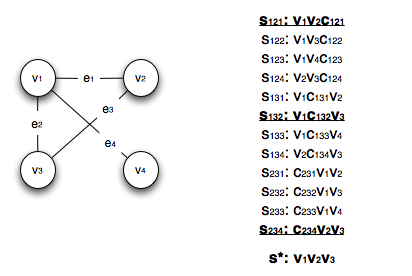
\includegraphics[width=\linewidth]{images/example}
\caption[An example showing the parameterized reduction from {\sc Clique} to {\sc CSWO}.]{An example of the parameterized reduction from a {\sc Clique} instance $G$ with $t = 3$ to an instance of {\sc CSWO} with 12 strings with $\ell = t = 3$, $d = t - 2 = 1$, and $n^* = {3 \choose 2} = 3$.  In bold we have the set of strings $S^* = \{s_{121}, s_{132}, s_{234}\}$ that corresponds to the clique containing the vertices $\{v_1, v_2, v_3\}$.  We note that $S^*$ is the only set of size 3 of strings with Hamming distance at most $d$ from the center string $s^*$. }
\label{fig:example}
\end{center}
\end{figure}

\subsection{Correctness of the Reduction}

The following two lemmas establish the correctness of the reduction. 

\begin{lemma} \label{direction_one_lemma} For a graph with a $t$-clique, the construction in Subsection \ref{w1_construction}  produces a {\sc CSWO} instance with a set $S^*$ and a string $s$ of length $\ell$ such that for every $s_i \in S^*$ $d(s_i, s) \leq d$. \end{lemma}

\begin{proof} Let the input graph have a clique of size $t$.  Let $v_{\alpha_1}, v_{\alpha_2}, \ldots, v_{\alpha_t}$ be the vertices in the clique $C$ of size $t$ and without loss of generality, assume $\alpha_1 < \alpha_2 < \ldots < \alpha_t$.  Then we claim that there exists a subset of ${t\choose 2}$ vertices that have distance at most $t - 2$ from the string $s = v_{\alpha_1} v_{\alpha_2} \ldots v_{\alpha_t}$.   Consider the first edge of the clique $(v_{\alpha_1}, v_{\alpha_2})$.  The string $s_{11r} = v_{\alpha_1} v_{\alpha_2} [c_{11r}]^{t - 2}$, where edge $r$ has endpoints  $v_{\alpha_1}$ $v_{\alpha_2}$, is contained in the set of strings $\{s_{111}, s_{112}, \ldots, s_{11|E|} \}$. Clearly, $H(s_{11r}, s) = t - 2$. For each edge in $C$ we have we have a string in $S$ that has distance at most $t - 2$ from $s$, as required.  \hfill $\Box$ \end{proof}

For the reverse direction, we need to prove that the existence of a subset $S^*$ of ${t \choose 2}$ and a string $s$ where $d(s, s_i) \leq t - 2$ for all $s_i \in S^*$ implies the existence of a clique in $G$ with $t$ vertices.  

\begin{lemma} \label{direction_two_lemma} If $(S, \ell, d, n, k)$ is a `YES' instance of the {\sc CSWO} problem then $(G, t)$ is a `YES' instance of the {\sc Clique} problem.  \end{lemma}

\begin{proof} Hence, we are required to show that the $t$ symbols of the center string correspond to the $t$ vertices of clique in the input graph.  Let $S^*$ be the subset of $S$ of size $t\choose 2$ such that $s$ has distance $t - 2$ from each string in $S^*$. Since $\ell = t$, $n^* = t$, $d = t -2$ and for each symbol $c_{i,j,m}$ there exists only a single string  $i = 1, \ldots, t$, $ j = 1, \ldots, t$ and $m = 1, \ldots, |E|$ it follows from the Pigeonhole principle that the center string $s$ only contains symbols from $\{v_i | \mbox{  for all } i = 1, \ldots, |V|\}$. Without loss of generality assume $s$ is equal to $v_{\alpha_1} v_{\alpha_2}\ldots v_{\alpha_t}$ for $\alpha_{v_1}, \alpha_{v_2}, \ldots, \alpha_{v_t} \in \{1, \ldots, |V|\}$. Consider any pair $\alpha_i, \alpha_j$ for $1 \leq i < j \leq t$ and consider the set of strings $S_{i,j} = \{ s_{i,j,1}, s_{i,j,2}, \ldots, s_{i,j,|E|} \}$.  Recall that $S_{i,j}$ contains a string corresponding to each edge $e = (r, s)$ in $E$ which has $v_r$ at the $i$th position and $v_s$ at the $j$th position and $c_{i,j,m}$ at all remaining positions.  Therefore, we can only find a string in $S_{i,j}$ that has distance at most $t - 2$ from $s$ if $v_{\alpha_i}$ is at the $i$th position and $v_{\alpha_j}$ is at the $j$th position; and such a string exists if and only if there is an edge in $G$ connecting $v_{\alpha_i}$ to $v_{\alpha_j}$. Hence, the center string $s$ implies there exists an edge between any pair of vertices in $G$ in the set $\{v_{\alpha_1} v_{\alpha_2}\ldots v_{\alpha_t}\}$ and by definition the vertices form a clique. \hfill $\Box$  \end{proof}

Our main theorem follows directly from Lemma \ref{direction_one_lemma} and Lemma \ref{direction_two_lemma}.  We note that the hardness for the combination of all three parameters also implies the hardness for each subset of the three. 

\begin{theorem} {\sc CSWO} with unbounded alphabet is W[1]-hard with respect to the parameters $\ell$, $d$, and $n^*$.\end{theorem}

Since there exists a trivial reduction from the {\sc Closest String} problem to {\sc CSWO} ({\em i.e.}\ simply set $k = 0$ in {\sc CSWO}), there cannot exist a fixed parameter tractable algorithm for {\sc CSWO} with $k$ as a parameter, unless P = NP; such an algorithm would contradict the NP-hardness of {\sc Closest String}. 

\begin{fact} {\sc CSWO} is W[1]-hard with respect to the parameter $k$, for any fixed $|\Sigma| \geq 2$. \end{fact}

%%%%%%%%%%%%%%%%%%%%%%%%%%%%%%%%%%%%%%%%%%%%%%%%%%%%%%%%%%%%%%%%%%%%%%%%%%%%%

\section{Summary and Open Problems}

We introduced the {\sc CSWO} problem, and proved that with unbounded alphabet size and parameterized by $\ell$, $d$ and $n^*$ it is W[1]-hard.  We also gave fixed parameter algorithms for the problem when parameterized by $d$ and $k$, and with unbounded alphabet size.  In the case of a fixed alphabet size, we showed {\sc CSWO} is fixed parameter tractable when parameterized by $n=n^*+k$. Table \ref{tab:results} summarizes these tractability and intractability results. Currently, the fixed parameter tractability of the {\sc CSWO} problem when parameterized by $d$, $n^*$ and $\Sigma$, and by $n^*$ and $k$, remains open (see Table \ref{tab:results}).  


\begin{table}
\begin{center}
\begin{tabular}{@{\hspace{0.5cm}}l  @{\hspace{0.5cm}}c @{\hspace{0.5cm}}c }
	\hline
  Parameter(s) 		 		& $|\Sigma|$ is a parameter  & $|\Sigma|$ is unbounded  \\
  \hline
  $\ell, d, n^*$ 			& FPT (trivial)							& W[1]-hard (*) \\  %% trivial
  $\ell$  						& FPT (trivial)							& W[1]-hard (*)\\ %% trivial
 % $d, n^*$ 					& FPT (*)									& W[1]-hard (*)\\ %% Follows from n^* being FPT
  %$n^*$ 						& Open									& W[1]-hard (*)	 \\ %% proof sketch  
  $d, n^*$ 					& Open										& W[1]-hard (*) \\
  $d, k$ 						& FPT (*)									& FPT (*) \\  %% proof sketch  
  $n^*, k$ 					& FPT									& Open \\   %% follows from n^* being FPT
  $k$ 							& W[1]-hard (trivial)					& W[1]-hard (trivial) \\ %% done   
  \hline
\end{tabular}\end{center}
\caption[An overview of the fixed parameter tractability and intractability of the {\sc CSWO}.]{An overview of the fixed parameter tractability and intractability of the {\sc CSWO}. Asterisk denotes the new results discussed in this chapter.}
\end{table}\label{tab:results}

In addition, the existence of efficient, non-trivial approximation algorithms for this problem warrants further investigation. Smith \cite{asmith} proved {\sc Maximum Coverage Approximation Substring} is APX-hard, however, the reduction does not directly extend to the specific case where $m = \ell$ ({\em i.e.}\ {\sc CSWO}).  Therefore, it currently remains open as to whether {\sc CSWO} is APX-hard.  He also proved that the $|\Sigma|^d$-approximation algorithm for {\sc Maximum Coverage Approximation Substring} provides a $(d + 1)$-relaxed decision procedure for {\sc CSWO}.  A $\rho$-decision procedure is an optimization algorithm that finds a solution with performance ratio $\rho$, or correctly concludes that no exact solution exists.  

There are many open problems concerning the approximability of  {\sc CSWO} and {\sc Maximum Coverage Approximation Substring}. As mentioned by Smith ``{\sc Maximum Coverage Approximation Substring} has a large margin for improvement in the complexity bounds'' \cite[page 80]{asmith}.  Among the problems outlined in this chapter, one of the key open problems is the development of a polynomial algorithm that gives a constant approximation guarantee, even for alphabets of constant size.  